\documentclass[a4j,11pt,twoside]{ujbook}
\usepackage{ascmac}
\usepackage[dvipdfmx]{graphicx}
\usepackage{matx}
\usepackage{manyfloat}
\begin{document}
%--------------------------------------------
% タイトルページ
\title{倒立振子の安定化制御}
\author{瀧川文哉}
\date{2017年7月}
\maketitle
%--------------------------------------------
% 目次
\pagenumbering{roman}
\tableofcontents
\listoffigures
\listoftables
\cleardoublepage
\pagenumbering{arabic}
%--------------------------------------------
% 本文
\chapter{はじめに}
\section{実験目的}
本実験の目的は倒立振子の安定化制御の制御系の設計を状態空間法を用いて行うことにより、線形時不変システムに対する設計法を習得することである。
\section{制御対象と制御目的}
\subsection{倒立振子系}
制御対象として、図\ref{fig:倒立振子系}に示されるような倒立振子系を考える。モノレール上に台車が置かれ、台車上のモノレールと直角な軸に一本の棒が取り付けられ、棒はその軸まわりに自由に回転できる。台車はベルトとプーリを介して、モータにより駆動され、モノレール上を走行できる。すなわち、棒(振子)は鉛直線とモノレールにより定まる平面に拘束されて、台車によって動かされるようになっている。

\subsection{観測出力と操作入力}
倒立振子系の観測出力として、ポテンショメータにより、次の2つが測定できる。
\begin{description}
	\setlength{\itemindent}{0pt}
	\item[1°] 台車の基準位置からの変位$r$に比例する電圧$y_1$
	\item[2°] 棒の鉛直線となす角度$\theta$に比例する電圧$y_2$
\end{description}
一方、操作入力は、つぎのものである。
\begin{description}
	\setlength{\itemindent}{0pt}
	\item[1°] モータの駆動アンプへの入力電圧$u$
\end{description}
ここで、モータにより駆動される台車には、$u$に比例した駆動力が働くものとする。
\subsection{制御目的}
この倒立振子系は、2つの平衡点をもつ。1つは棒が鉛直線に沿って垂れ下がった状態、もう一つは棒が鉛直線に沿って倒立した状態である。前者は、棒を揺らせば、いわゆる振子となり、揺らせれば、いわゆる振子となり、ゆれは時間が立てば止まるので、安定平衡点である。後者は、いわゆる倒立振子であるが、倒立状態にある棒を少しでもつつけば、真っ逆さまに落ちていくので、不安定平衡点である。このような倒立振子系に対する制御目的として、つぎを考える。
\begin{description}
	\setlength{\itemindent}{0pt}
	\item[1゜]倒立状態にある棒が何らかの原因で傾いたとき、台車を動かして、棒をすみやかに倒立状態に戻す(不安定抵抗店の安定化)。
	\item[2゜]倒立位置を指定した位置に移動させる。
\end{description}
% 1.1図の挿入
\begin{figure}[htbp]
	\begin{center}
		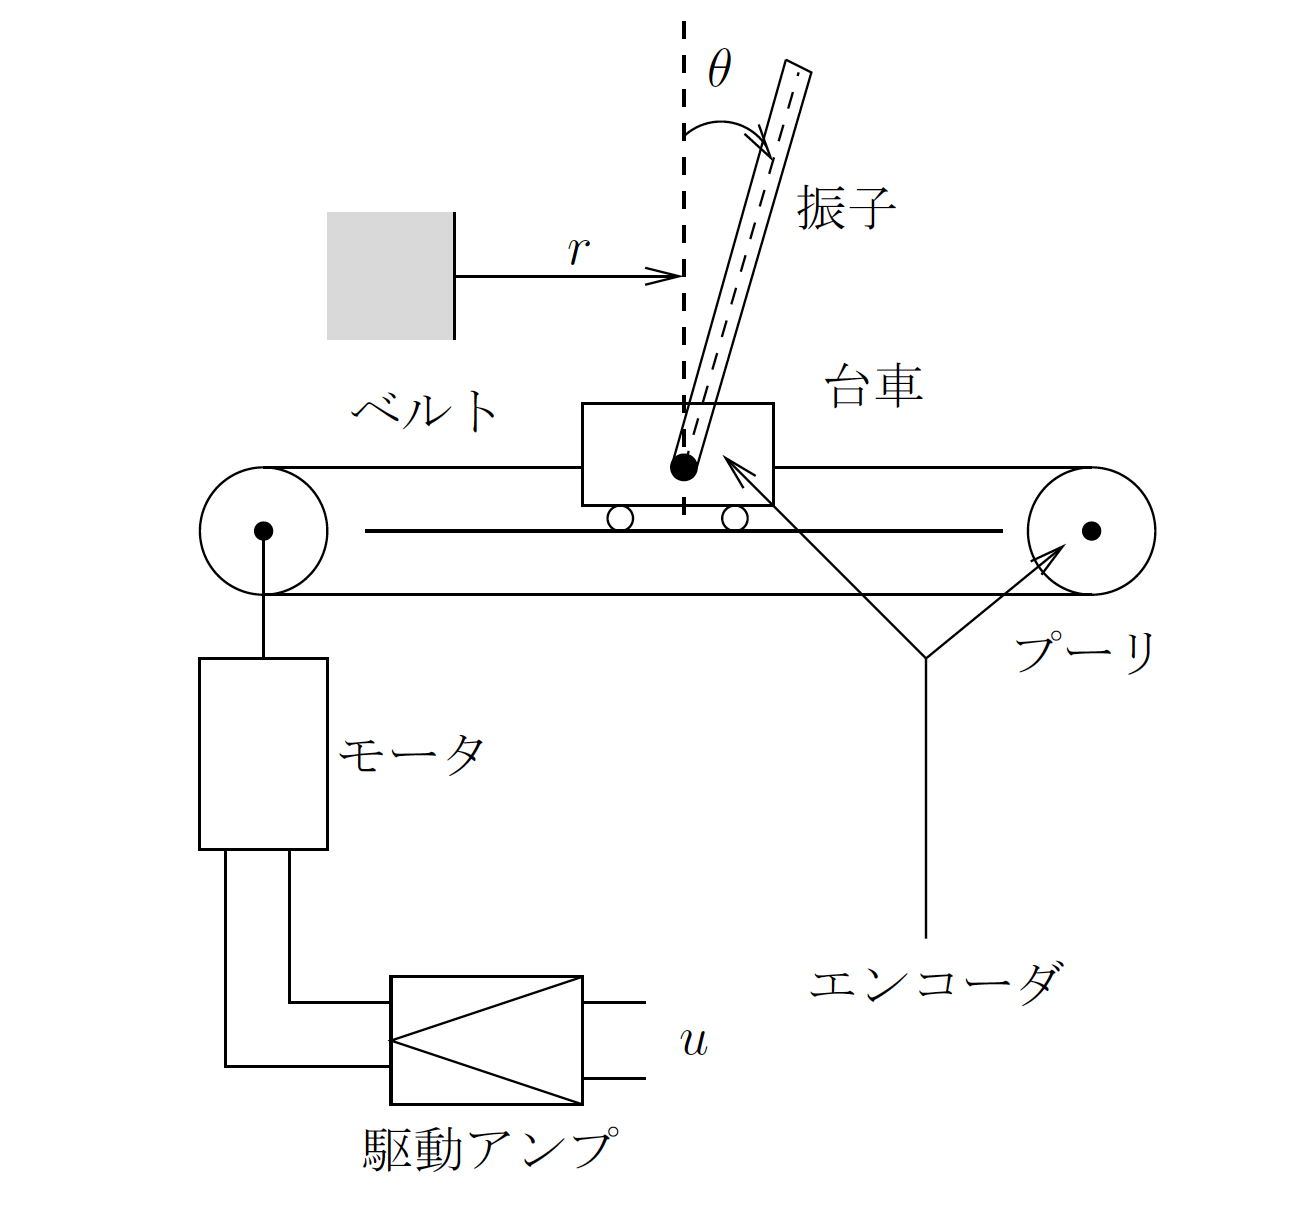
\includegraphics[width = 0.6 \linewidth]{model.png}
		\caption{倒立振子系}
		\label{fig:倒立振子系}
	\end{center}
\end{figure}

\chapter{モデリング}
\section{数式モデル}
制御目的を達成する制御システムを設計するためにまず、倒立振子系について、状態方程式と観測方程式から成る数式モデルを導出する。
\subsection{状態方程式}
% 2.1図の挿入
\begin{figure}[htbp]
	\begin{center}
		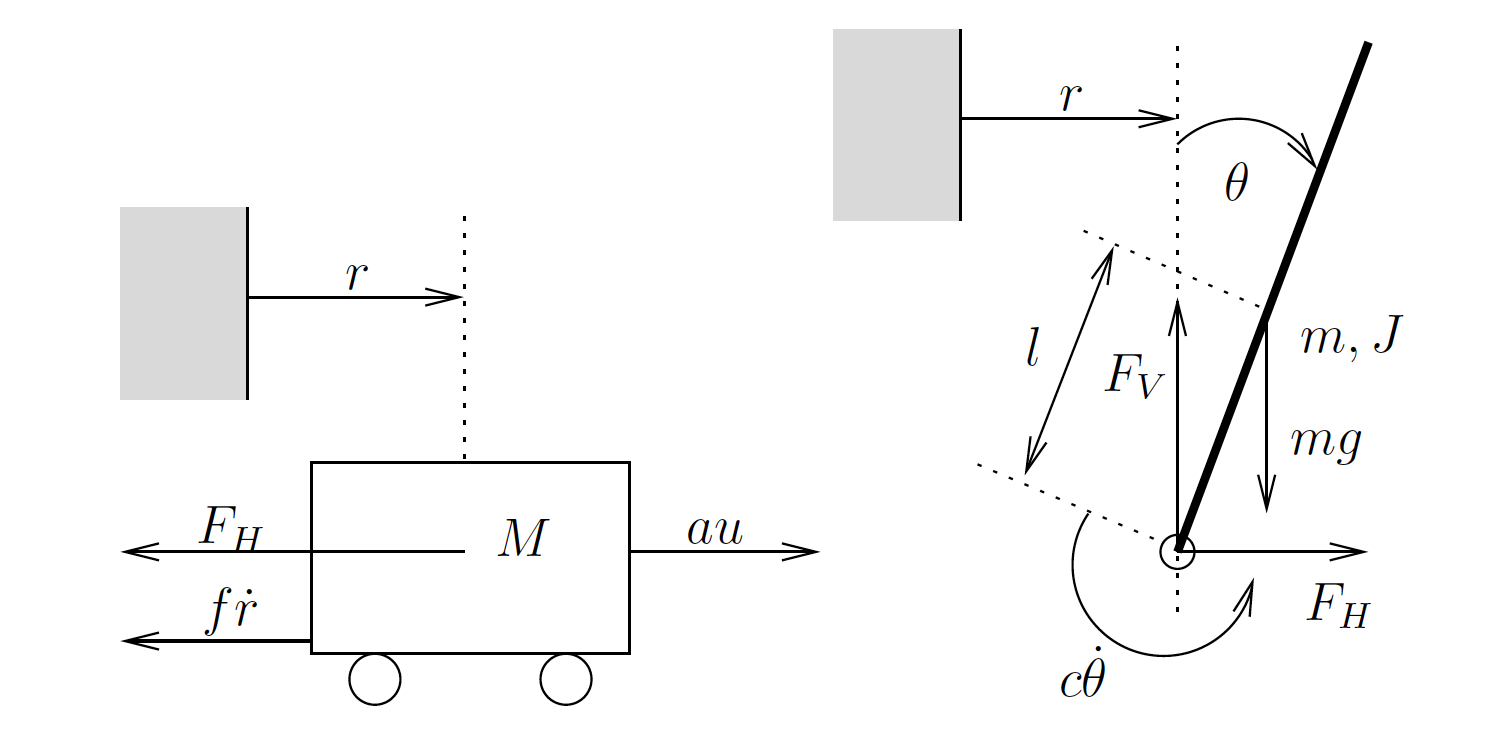
\includegraphics[width = 0.6 \linewidth]{modeling.png}
		\caption{数学モデル導出のための参考図}
		\label{fig:数式モデル導出のための参考図}
	\end{center}
\end{figure}

図\ref{fig:数式モデル導出のための参考図}を参照して、台車と振子に関する運動方程式がつぎのように得られる。

\begin{eqnarray}
&&M \ddot{r} = au - F_H - f \dot{r}
\label{eq:2.1}\\
&&J \ddot{\theta} = lF_V\sin{\theta} - lF_H\cos{\theta} - c\dot{\theta}
\label{eq:2.2}\\
&&m \frac{d^2}{dx^2} (r + l\sin(\theta))  =  F_H
\label{eq:2.3}\\
&&m \frac{d^2}{dx^2} (l\cos(\theta))  =  F_V - mg
\label{eq:2.4}
\end{eqnarray}
ここで、$M,f$は台車の質量と摩擦係数、$m,l,J,c$は振子の質量、回転軸・重心間距離、重心まわり慣性モーメント、回転軸摩擦係数、$F_H,F_V$は振子が台車から受ける水平抗力と垂直抗力である。また、$u$は駆動アンプへの入力電圧、$a$は駆動アンプへの入力電圧から台車への駆動力までのゲインである。

いま、4つの状態変数から成るベクトル、すなわち状態$x$を
\begin{eqnarray*}
	x=\left[
	\begin{array}{c}
		r\\
		\theta\\
		\dot{r}\\
		\dot{\theta}
	\end{array}
	\right]
\end{eqnarray*}
のように定義すると、、(\ref{eq:2.1})-(\ref{eq:2.4})式から、倒立振子系の非線形状態方程式を求める。
(\ref{eq:2.1})に(\ref{eq:2.2})を代入すると

\begin{eqnarray*}
	M\ddot{r} = au - m\ddot{r}+ml\sin{\theta}-f\dot{r}
\end{eqnarray*}
\begin{eqnarray}
\ddot{r} = \frac{au + ml\sin{\theta}-f\dot{r}}{M+m}
\label{eq:rddot}
\end{eqnarray}
また、(\ref{eq:2.2})に(\ref{eq:2.3}),(\ref{eq:2.4})を代入すると
\begin{eqnarray*}
	J\ddot{\theta} = l\left(m\frac{d^2}{dt^2}(l\cos{\theta}+mg) \right)\sin{\theta}
	- l \left( m\frac{d^2}{dt^2}(r+l\sin{\theta}) \right)\cos{\theta}
\end{eqnarray*}
\begin{eqnarray}
ml\cos{\theta}\ddot{r}+(J+ml^2)\ddot(\theta)=mgl\sin{\theta}-c\dot{\theta}
\label{eq:rddot,thddot}
\end{eqnarray}
(\ref{eq:rddot}),(\ref{eq:rddot,thddot})を行列式で表すと
\begin{eqnarray*}
	\left[
	\begin{array}{cc}
		M+m & ml\cos{\theta}\\
		ml\cos{\theta} & J+ml^2
	\end{array}
	\right]
	\left[
	\begin{array}{c}
		\ddot{r} \\
		\ddot{\theta}
	\end{array}
	\right] =
	\left[
	\begin{array}{c}
		- f \dot{r} + ml\sin{\theta}・\dot{\theta}^2 + au\\
		mgl\sin{\theta} - c\dot{\theta}
	\end{array}
	\right]\\
	\left[
	\begin{array}{c}
		\ddot{r} \\
		\ddot{\theta}
	\end{array}
	\right] =
	\left[
	\begin{array}{cc}
		M+m & ml\cos{\theta}\\
		ml\cos{\theta} & J+ml^2
	\end{array}
	\right]^{-1}
	\left[
	\begin{array}{c}
		- f \dot{r} + ml\sin{\theta}・\dot{\theta}^2 + au\\
		mgl\sin{\theta} - c\dot{\theta}
	\end{array}
	\right]
\end{eqnarray*}
よって、
%(5)
\begin{eqnarray}
\dot{x}=f(x,u)=\left[
\begin{array}{c}

\dot{r}\\
\dot{\theta}\\
K^{-1}\left[
\begin{array}{c}
- f \dot{r} + ml\sin{\theta}・\dot{\theta}^2 + au\\
mgl\sin{\theta} - c\dot{\theta}
\end{array}
\right]

\end{array}
\right],\,
K = \left[
\begin{array}{cc}
M+m & ml\cos{\theta}\\
ml\cos{\theta} & J+ml^2
\end{array}
\right]
\end{eqnarray}
のように得られる。

ところで、倒立振子系については、その制御目的から、不安定平衡点$x=0$の近傍での挙動を表す方程式を知れば充分である。そこで、この基準状態まわりで一次近似された状態方程式を求めることを考える

倒立振子系に対する状態方程式は、つぎのように得られる。
%(6)
\begin{eqnarray}
\dot{x} = Ax + Bu
\label{eq:xdot}
\end{eqnarray}
\noindent
ここで

\begin{eqnarray*}
	A = \left[
	\begin{array}{cc}
		0_{2×2} & I_2\\
		A_{21} & A_{22}
	\end{array}
	\right],\,
	B = \left[
	\begin{array}{c}
		0_{2×2}\\
		B_2
	\end{array}
	\right]\\
\end{eqnarray*}
\noindent
ただし

\begin{eqnarray*}
	A_{21} = K^{-1}\left[
	\begin{array}{cc}
		0 &  0 \\
		0 & mgl
	\end{array}
	\right],\,
	A_{22} = K^{-1}\left[
	\begin{array}{cc}
		-f &  0 \\
		0 & -c
	\end{array}
	\right],\,
	B_{2} = K^{-1}\left[
	\begin{array}{c}
		a\\
		0
	\end{array}
	\right]
\end{eqnarray*}

\begin{eqnarray*}
	K = \left[
	\begin{array}{cc}
		M+m & ml \\
		ml & J+ml^2
	\end{array}
	\right]
\end{eqnarray*}

\subsection{観測方程式}
2つの観測出力は
\begin{eqnarray*}
	y_1 &=& c_1r\\
	y_2 &=& c_2\theta
\end{eqnarray*}
のように表される。ここで$c_1$は変位・電圧変換係数、$c_2$は角度・電圧変換係数である。これから成るベクトルすなわち出力$y$を

\begin{eqnarray*}
	y = \left[
	\begin{array}{c}
		y_1\\
		y_2
	\end{array}
	\right]
\end{eqnarray*}
のように定義すると、倒立振子系に対する観測方程式として

\begin{eqnarray*}
	y = Cx
\end{eqnarray*}
ただし

\begin{eqnarray}
C = \left[
\begin{array}{cc}
N & 0_{2×2}
\end{array}
\right] = \left[
\begin{array}{cccc}
c_1 &  0  & 0 & 0\\
0  & c_2 & 0 & 0
\end{array}
\right],\,
N = \left[
\begin{array}{cc}
c_1 &  0 \\
0  & c_2
\end{array}
\right]
\label{eq:C,N}
\end{eqnarray}
を得る。

\section{物理パラメータの決定}
\section{パラメータの検証}

\chapter{制御系設計}
\begin{figure}

\end{figure}
\section{特性解析}
\section{制御システムの構成}
\section{$F$の設計}
\section{$\hat{A}$,$\hat{B}$,$\hat{J}$,$\hat{C}$,$\hat{D}$の設計}
\section{離散化}
\section{振り上げ制御}	

\chapter{シミュレーション}
\section{安定化制御}
\section{振り上げ制御}

\chapter{実験}
\section{実験装置}
\section{安定化制御}
\section{振り上げ制御}
\section{考察}

\chapter{おわりに}

\end{document}